\chapter{Grundlagen}

\section{Die \acrlong{fll}}
Bei der \acrlong{fll}(\acrshort{fll}) handelt es sich um Wettbewerbe, die von einer Kooperation von \gls{Lego} und \gls{First} organisiert werden. Das Ziel dieser Wettbewerbe ist es Kinder und Jugendliche für eine Laufbahn im \gls{MINT}-Bereich zu motivieren. In Zentraleuropa wird die \acrshort{fll} von dem Verein HANDS on TECHNOLOGY e.V. betrieben.\\
Mittlerweile besteht die \acrshort{fll} aus zwei Wettbewerben. Die \acrlong{fll} Explore für Kinder im Grundschulalter (6-10 Jahre) und die \acrlong{fll} Challenge für Kinder und Jugendliche der weiterführenden Schulen. Diese beiden Wettbewerbe haben ein gemeinsames Saisonthema, welches in dieser Saison (2021/22) das Thema \textit{Transport} war.\\

\subsection{Der Ablauf der \acrshort{fll} Explore} \label{preparation}
In der Vorbereitungszeit wird den Kindern von der \acrshort{fll} Explore ein IngenieurInnen Notizbuch und ein Motivationsset mit \gls{Lego}-Teilen zugeschickt. In diesem Notizbuch gibt es für jedes Treffen eine Seite mit Fragen und Aufgaben zum Saisonthema. Gelegentlich wird als Aufgabe auch ein Projekt aus der Projektbibliothek \ref{Projektbibliothek} gestellt. Die Aufgaben in dem Notizbuch drehen sich jedoch generell eher um das kreative Bauen, wie \textit{entwirf ein Transportmittel für das Wasser}, als um bewegliche und programmierbare Modelle. Somit nimmt das Programmieren in der Vorbereitung auf die \acrshort{fll} eine etwas untergeordnete Rolle ein.\\
Zuletzt wird von den Teams gefordert, ein Teammodell zu entwerfen, welches sie am Wettbewerbstag den Richtern vorführen und präsentieren. Hierzu soll ebenfalls ein Teamposter erstellt werden.


\section{Das Baukastensystem LEGO WeDo2.0} \label{Wedo}
Zur Durchführung der Kurse wurde der Baukasten LEGO WeDo 2.0 verwendet. Dessen Eigenschaften und Konzepte sollen hier erläutert werden.
\subsection{Das Konzept des Baukastens}
Die LEGO WeDo Produktreihe zielt darauf ab, Kindern spielerisch Inhalte der Naturwissenschaft und Technik, sowie grundlegende Programmierkonzepte zu vermitteln. Hierfür werd von LEGO Handbücher für Lehrer, Leitfäden sowie die Software mit der die Elektronischen Bauteile programmiert werden können zur Verfügung gestellt. Somit richten sich die Baukästen speziell an Schulen und andere Bildungseinrichtungen. Zu den Baukästen gibt es jeweils ein äquivalentes Produkt für zuhause, welches jedoch weniger technische Bauteile (Balken, Achsen, Zahnräder) sondern mehr bunte und dekorative Bauteile enthält.\\ 
Der Vorgänger des WeDo 2.0 Baukastens musste noch über ein USB Kabel direkt mit dem Computer verbunden sein. Des weiteren, enthielt dieser lediglich einen Motor, dessen Drehrichtung und Geschwindigkeit vom Computer aus eingestellt werden konnte. Aufgrund der benötigten USB Verbindung war es nicht möglich die Modelle von Tablet-Computern oder Smartphones zu steuern.  \\
Dahingegen verfügt der verwendete WeDo 2.0 Baukasten über zwei Sensoren und einen Motor. Des weiteren wird keine USB Verbindung mehr benötigt, sondern der Programmierbare Baustein über Bluetooth angesteuert. Durch die App kann neben einem normalen Computer auch über einen Tablet-Computer oder ein Smartphone programmiert werden.

\begin{figure}[htbp!]
	\centering
	\fbox{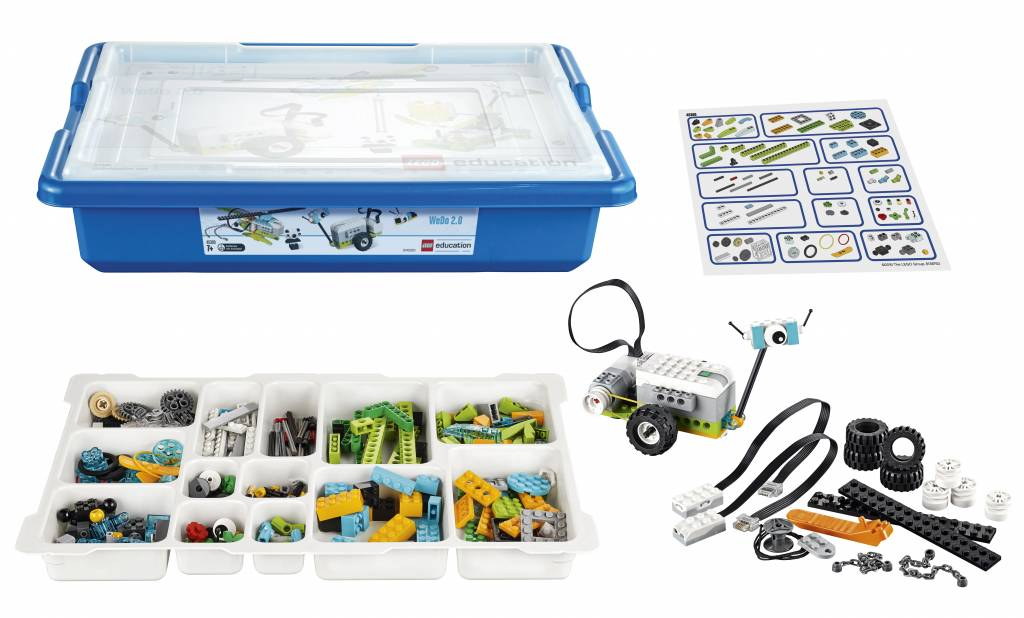
\includegraphics[width=0.4\textheight,angle=0]{img/lego-education-wedo-20}}
	\caption[Der WeDo 2.0 Baukasten]{Der WeDo 2.0 Baukasten} % \cite{knowAndLove}
	\label{img:lego-education-wedo-20}
\end{figure} 

\subsection{Inhalt}

\subsection{Die Projektbibliothek}\label{Projektbibliothek}
Das Programm zu dem WeDo 2.0 Baukasten bietet eine Projektbibliothek (Abb. \ref{img:projects}). Die Projekte innerhalb dieser haben alle einen ähnlichen Aufbau. Das Thema der Projekte ist aus dem \gls{MINT}-Bereich. Zu diesem werden den Kindern zunächst einige Fragen gestellt. Anschließend können sich die Kinder ein kleines Video zu dem Thema ansehen, welches die Kinder auf das Thema einstimmen soll. Beispielsweise ist in dem Video zum Thema \textit{Standfestigkeit} eine Erdkugel mit Kontinentalplatten, ein Seismograph, Aufnahmen von Erdbeben und verschiedene Gebäude, wie Hochhäuser und Pyramiden, zu sehen.\\
Anschließend dürfen die Kinder das Modell zu dem Thema bauen. Das in \ref{img:subject} gezeigte Modell zum Thema \textit{Standfestigkeit} stellt einen vereinfachten Erdbebensimulator dar, mit drei Modellgebäuden.\\
\begin{figure}[htbp!]
	\centering
	\fbox{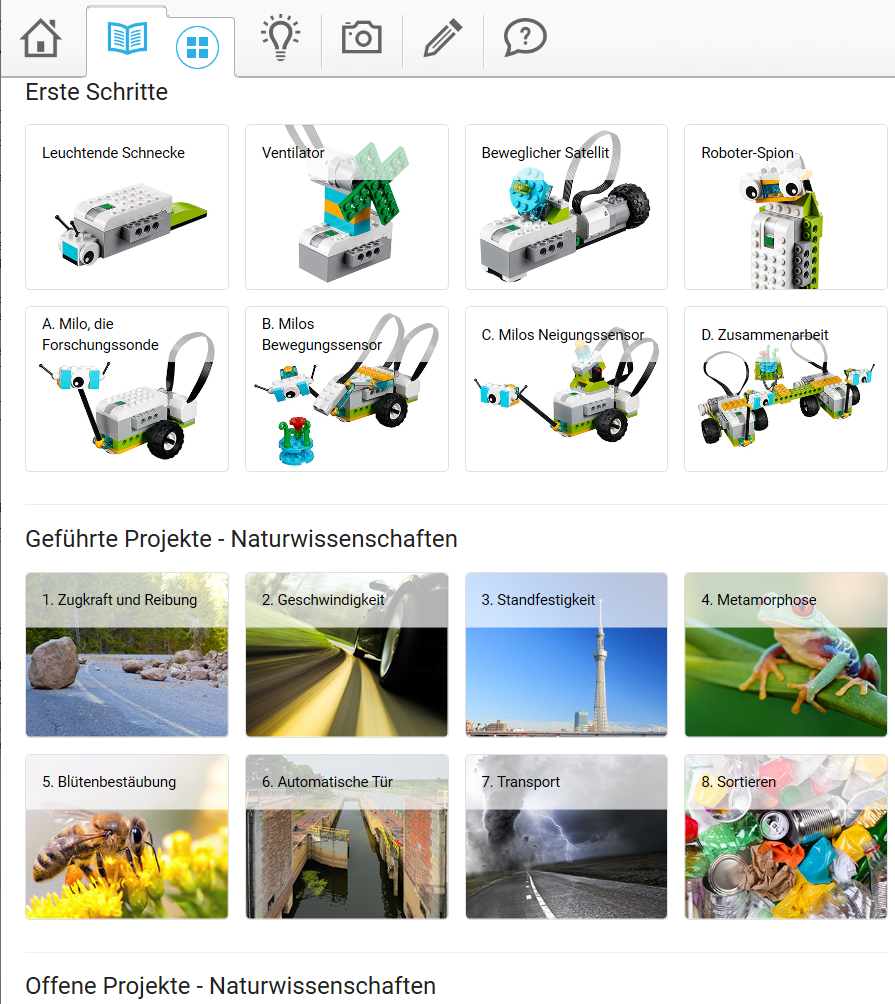
\includegraphics[width=0.4\textheight,angle=0]{img/Projects.png}}
	\caption[Die Programmbibliothek]{Die Programmbibliothek}
	\label{img:projects}
\end{figure} 

\begin{figure}[htbp!]
	\centering
	\fbox{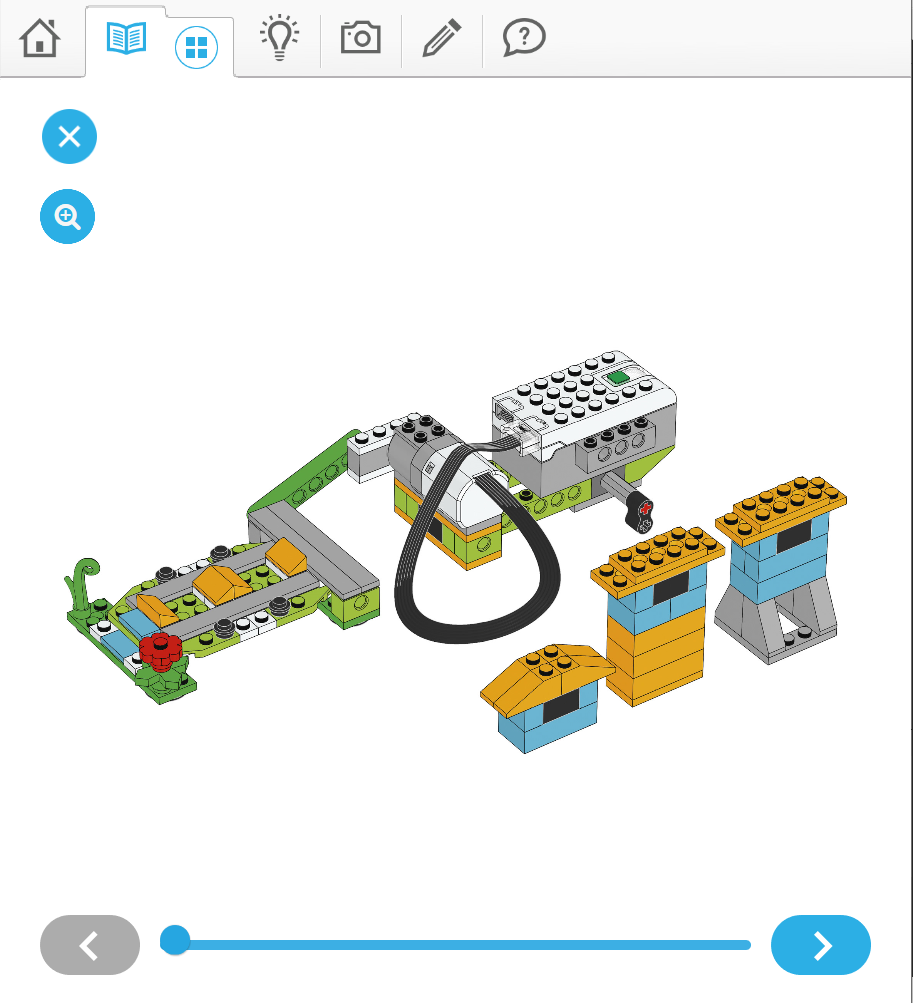
\includegraphics[width=0.4\textheight,angle=0]{img/Model.png}}
	\caption[Das Modell zum Thema Standfestigkeit]{Das Modell zum Thema \textit{Standfestigkeit}}
	\label{img:subject}
\end{figure} 

Nach dem Bau wird das Modell von den Kindern programmiert. Hierzu steht den Kindern eine Programmvorlage zur Verfügung, welche sie nachbauen können. Diese ist für das Projekt \textit{Standfestigkeit} in \ref{img:programtemplate} zu sehen. Dabei wird Motorgeschwindigkeit, welche die Erdbebenstärke simuliert, bei jedem Durchlauf um eins erhöht und der Motor für zwei Sekunden gedreht.\\
Daraufhin sollen die Kinder das Modell mit dem Programm ausprobieren.\\
Zum Abschluss kann den Kindern noch eine Kompetitive Aufgabe gegeben werden, bei der sie das Modell und Programm verbessern sollen. Bei dem Thema Standfestigkeit ist das die Aufgabe, ein Gebäudemodell zu entwerfen, welches der größten Erdbebenstärke standhält und gleichzeitig am höchsten ist.

\begin{figure}[htbp!]
	\centering
	\fbox{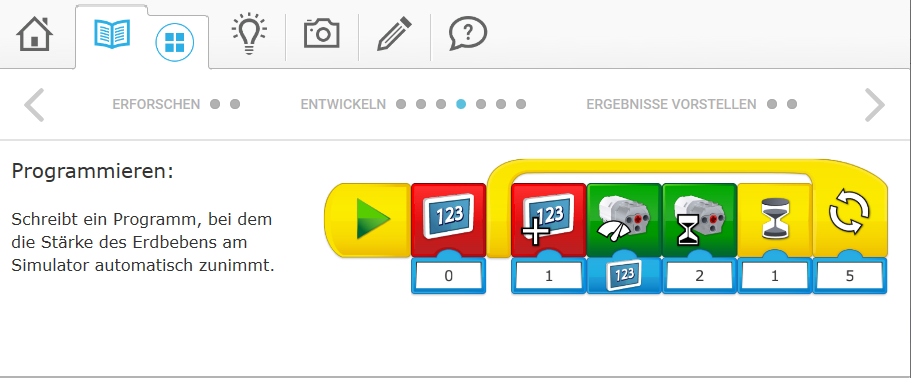
\includegraphics[width=0.4\textheight,angle=0]{img/programtemplate.png}}
	\caption[Die Programmvorlage]{Die Programmvorlage bei dem Thema \textit{Standfestigkeit}}
	\label{img:programtemplate}
\end{figure} 

\subsection{Programmieren mit WeDo 2.0}\label{WedoSoftware}
Um für Kinder leichter greifbar zu sein, wurde zum programmieren der Modelle eine Oberfläche gewählt, bei der einzelne Programmblöcke hintereinander gezogen werden. Die Abfolge der Blöcke ergibt damit das fertige Programm. Nach ihrer jeweiligen Funktion lassen sich die Programmblöcke in Kategorien einteilen. Eine Einteilung ist von LEGO durch die Farbgebung der Programmblöcke bereits gegeben. \\
Einige Blöcke benötigen einen zusätzlichen Wert, der ihnen übergeben werden muss. Diese sind mit einer halbkreisförmigen Öffnung an der Unterseite versehen. Die Blöcke, welche diese Werte liefern, hingegen sind mit einer halbkreisförmigen Wölbung versehen. 

\subsubsection{Die Aktionsblöcke}
\begin{figure}[htbp!]
	\centering
	\fbox{\includegraphics[width=0.4\textheight,angle=0]{img/Aktionsblöcke.png}}
	\caption[Die Aktionsblöcke]{Die Aktionsblöcke} % \cite{knowAndLove}
	\label{img:Aktionsblöcke}
\end{figure}

Mit den Aktionsblöcken Abb. \ref{img:Aktionsblöcke} können Motoraktionen und die Farbe der Statusleuchte gesteuert werden. Für den Motor kann einerseits die Richtung in welche sich der Motor dreht, die Geschwindigkeit und die Dauer der Motordrehung gesteuert werden.

\subsubsection{Die Arithmetik- und Medienblöcke}
\begin{figure}[htbp!]
	\centering
	\fbox{\includegraphics[width=0.4\textheight,angle=0]{img/LogikProgrammblöcke.png}}
	\caption[Die Arithmetik und Medienblöcke]{Die Arithmetik und Medienblöcke} % \cite{knowAndLove}
	\label{img:ArithmetikUndMedienblöcke}
\end{figure}
Mangels einer besseren Bezeichnung für diese Kategorie werden deren Blöcke hier als  Arithmetik- und Medienblöcke bezeichnet (Abb. \ref{img:ArithmetikUndMedienblöcke}). Es können einerseits Geräusche und Töne abgespielt werden. In der Bibliothek stehen 28 unterschiedliche Tonaufnahmen zur Verfügung. Ebenfalls können Bilder auf dem Bildschirm angezeigt werden. Die Tonaufnahmen und Bilder aus der Bibliothek passen jeweils Thematisch zu den Projekten aus der Projektbibliothek \ref{Projektbibliothek}. Die Bibliothek kann jedoch durch eigene Tonaufnahmen und Bilder ergänzt werden. Die Bilder und Tonaufnahmen werden von dem Gerät aus abgespielt, über welches das Modell programmiert wird, da der programmierbare Legostein, der die Befehle von dem Master-Gerät entgegennimmt, weder über ein Display, noch über Lautsprecher verfügt.\\
Mit den beiden Arithmetikblöcken können einfache Berechnungen durchgeführt werden. Es kann lediglich ein einziger Wert als Variable existieren. Dieser wird auf dem Bildschirm als große Zahl angezeigt. Das erlaubt die Beobachtung des Wertes, während der Programmausführung. Zur Verfügung stehen die Operationen: \textit{Plus}, \textit{Minus}, \textit{Mal} und \textit{Geteilt durch}.\\
Mit dem letzten Block dieser Kategorie (ganz rechts) kann das Bild und die Variable die angezeigt wird vergrößert oder verkleinert werden.

\subsubsection{Die Programmablaufblöcke}
\begin{figure}[htbp!]
	\centering
	\fbox{\includegraphics[width=0.4\textheight,angle=0]{img/Programmablaufblöcke.png}}
	\caption[Die Programmablaufblöcke]{Die Programmablaufblöcke} % \cite{knowAndLove}
	\label{img:Programmablaufblöcke}
\end{figure}
In Abb. \ref{img:Programmablaufblöcke} sind die Blöcke zu sehen, welche den Programmablauf steuern. Bei den drei linken Blöcken handelt es sich um die verschiedenen Startblöcke.\\
Der mit dem grünen Pfeil erlaubt den Start eines dahinterliegenden Programmteils mittels eines einfachen Knopfdrucks. Mit dem zweiten Block kann der Programmteil durch einen Buchstaben der Tastatur gestartet werden. Der Buchstabe mit dem das Programm gestartet wird, kann für jeden einzelnen dieser Blöcke geändert werden, sodass ein leichtes Auswählen verschiedener Programmteile ermöglicht wird.\\
Der dritte Startblock mit dem Briefumschlag, der in einen Briefkasten geworfen wird, als Symbolbild kann ein Programm durch ein Signal aus einem anderen Programmteil gestartet werden. Das Signal wird von dem Block rechts daneben gesendet, mit dem Briefumschlag als Symbolbild. Diesem wird ein Wert übergeben und anschließend wird der Startblock gestartet, der den gleichen Wert hat. \\
Der Block mit der Sanduhr dient dazu, eine bestimmte Zeit zu Warten. Er kann jedoch auch dafür verwendet werden, auf einen Sensorzustand zu warten. Ein kleines Beispiel zu dem Programmstart mit dem Postkasten-Block und dem Warten-Block ist in Abb. \ref{img:Beispiel_01} zu sehen. Dabei wird nach Starten des Programms durch den grünen Pfeil, zunächst der obere Programmteil gestartet, welcher den Motor nach rechts drehen lässt und nach einer Sekunde der untere Programmteil, der den Motor nach links drehen lässt. 



\begin{figure}[htbp!]
	\centering
	\fbox{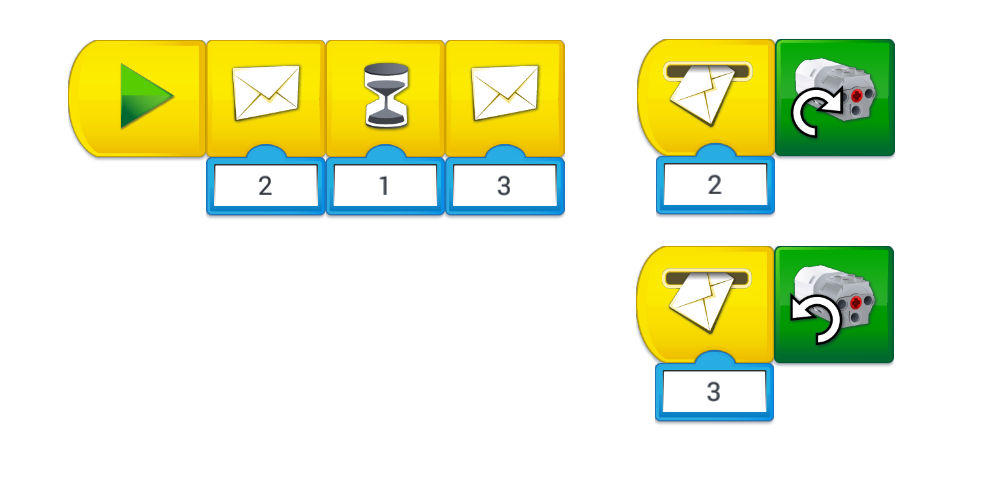
\includegraphics[width=0.4\textheight,angle=0]{img/Example_01.png}}
	\caption[Beispielprogramm zum Start aus anderem Programmteil]{Beispielprogramm zum Start aus anderem Programmteil} % \cite{knowAndLove}
	\label{img:Beispiel_01}
\end{figure}

\subsubsection{Wertblöcke}

Die Blöcke, welche zusätzliche Werte zur Konfiguration benötigen können über die Wertblöcke andere Werte zugewiesen bekommen. Diese Art Blöcke wird in die halbkreisförmige Öffnung des Blockes gehängt, dem ein neuer Wert zugewiesen werden soll. \\
Zur Verfügung stehen Zahlenwerte, Zeichenketten, die Variable vom Bildschirm und ein zufälliger Zahlenwert zwischen 0 und 10.

\begin{figure}[htbp!]
	\centering
	\fbox{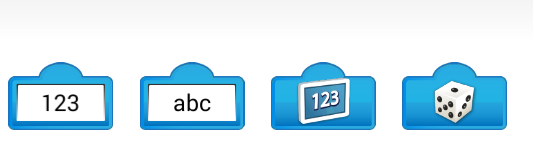
\includegraphics[width=0.4\textheight,angle=0]{img/Werte.png}}
	\caption[Werte]{Werte}
	\label{img:Werte}
\end{figure}


\subsubsection{Sensorwertblöcke}

Diese Blöcke werden verwendet, um Blöcken einem Sensorwert zuzuweisen. Die Blöcke können Werte zwischen 0 und 10 annehmen und bilden somit ihre Messwerte auf dieser Skala ab.\\
Der Kippsensor weist jeder Kipprichtung einen Ganzzahlwert zu. Damit kann eine Hebelsteuerung realisiert werden. \\
Der Distanzsensor misst grob eine Distanz zu Hindernissen. Damit kann Beispielsweise ein Automodell vor einer Wand zum stehen gebracht werden.\\
Der Lautstärkesensor misst grob die Umgebungslautstärke. Damit kann ein Programm durch klatschen gestartet werden.

\begin{figure}[htbp!]
	\centering
	\fbox{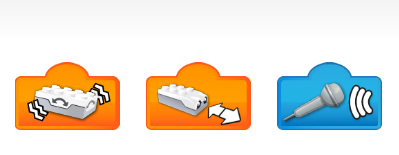
\includegraphics[width=0.4\textheight,angle=0]{img/Sensoren.png}}
	\caption[Sensorwerte]{Sensorwerte} % \cite{knowAndLove}
	\label{img:Sensorwerte}
\end{figure}


\section{Die Kurse}
Durchgeführt wurden grundsätzlich zwei Arten der Kurse. Die Erste fand hauptsächlich in der Zeit Anfangszeit statt, jedoch auch während der Zeit in der aufgrund der Corona-Lage ausschließlich online Kurse möglich waren. Die Aufgabe bestand darin, die Kinder mit dem Baukasten \ref{Wedo} vertraut zu machen. Dabei wurden als Grundlage für diese Kurse die Projektbibliothek \ref{Projektbibliothek} verwendet. Es standen hauptsächlich das Programmieren und Verbessern eines vorgegebenen Modells im Vordergrund. Durch die kompetitive Aufgabe, die bei diesen Projekten immer in der zweiten Hälfte kam, konnten die Kinder bis zum Schluss motiviert gehalten werden. Dies war online leider nicht möglich.\\
Die Zweite fand im Kontext der Vorbereitung auf die \acrlong{fll} statt. Diese wurden nach dem IngenieurInnen Notizbuch durchgeführt \ref{preparation}. Es stand viel das kreative Bauen, die Auseinandersetzung mit dem Saisonthema und mit den Grundwerten (Entdeckung, Inklusion, Innovation, Teamwork, Wirkung und Spaß) im Vordergrund. 





\section{Myers-Briggs-Typenindikator\textsuperscript{\textregistered}} 
\subsection{Typen nach Jung}
Der Psychoanalytiker Carl Gustav Jung definierte im 20. Jahrhundert insgesamt acht verschiedene Typen. Diese Typen sind unterteilt in zwei Kategorien mit je vier Typen. Die beiden Kategorien, die Jung definierte, sind die Kategorie \glqq Extrovertiert"' und \glqq Introvertiert"'. In beiden Kategorien sind jeweils die vier Typen Fühlend, Denkend, Intuitiv und Empfindend. \cite{jung_1921}\\

In den folgenden Abschnitten werden mithilfe des Werks \citetitle{jung_2014} Jungs Kategorien sowie die Typen kurz zusammengefasst.
\subsubsection{Extrovertiert}
Nach \citeauthor{jung_2014} sind Menschen, welche in Jungs Kategorie der Extravertierung
fallen, sehr lebhafte Menschen, die den Kontakt zu Anderen lieben. Wenn extravertierte Menschen sich an eine Gruppe anpassen müssen, fällt ihnen das sehr einfach. Menschen, die als extravertiert bezeichnet werden, werden häufig als störend bezeichnet. Ihrer eigenen Innenwelt wird von diesen Menschen nur wenig Achtung geschenkt, was sie als eher oberflächliche Menschen wirken lässt. Wenn es um Tätigkeiten geht, übernehmen extravertierte Menschen Rollen, welche organisatorischer, kreativer oder repräsentativer Art sind. 

\noindent
\cite{jung_2014}

\subsubsection{Introvertiert}

Introvertierte Menschen sind das Gegenteil der Extrovertierten. Sie scheuen den Kontakt mit der Außenwelt und sind dadurch viel mehr auf ihr Inneres fokussiert. Diese Menschen zeigen nach dem Autor \citeauthor{jung_2014} des Werks \citetitle{jung_2014} häufig scheue und verschlossene Charakterzüge, seltener auch etwas weltfremde Züge. Dieser Typus von Menschen neigt nach dem Autor auch häufig zu Rechthaberei und Eigensinn, woraus Konflikte resultieren. Im Vergleich zu den eher praktischen Aufgaben, die extravertierte Menschen lieben, bevorzugen introvertierte Menschen eher die theoretischen Aufgaben.

\noindent
\cite{jung_2014}

\subsubsection{Fühlend}
Offenheit, Toleranz und Teamfähigkeit sind Eigenschaften, die nach Hans Jung und C. G. Jung dem extravertierten fühlenden Typus zugesprochen werden. Als charakterliche Züge werden diese Menschen als loyal und treu beschrieben. Da sich der extravertierte Typus weniger auf seine Innenwelt, sondern eher auf die Außenwelt fokussiert, beschränken sich auch die Gefühle des extravertierten Fühltypus nicht nur auf seine Innenwelt.\\
Sollte der Mensch sich mit seinen Gefühlen weniger auf die Außen-, sondern auf die Innenwelt beschränkt, handelt es sich um einen introvertierten Fühltypus. Die Urteilsbildung eines solchen Menschens werden von seinen eigenen persönlichen Werten geleitet. 

\noindent
\cite{jung_2014}
\subsubsection{Denkend}
\citeauthor{jung_2014} fasst den extravertierten Denktypus nach \citeauthor{jung_1921} als eine Person, welche sich analytisch mit seiner Welt auseinandersetzt und Bewertungen und Beurteilungen auf eine sachliche Weise durchgeführt werden. Das Treffen von Entscheidungen ist keine Hürde für extravertierte Menschen des Denktypus. Personen dieses Typs übernimmt wie bereits erwähnt gerne Tätigkeiten organisatorischer Art, da es in dessen Natur liegt zu versuchen, seine Umwelt zu organisieren.\\
Personen, welche dem introvertierten 



Der introvertierte Denktypus hingegen lässt sich nur mit Tatsachen überzeugen. 
Er denkt und handelt logisch, objektiv, kritisch und unpersönlich. Er versucht nicht 
seine Umwelt zu ändern oder ihr seine Ideen aufzudrängen. Negativ für einen solchen Typus ist, dass seine Gedankengänge für andere Personen schwer verständlich 
sind und diese ihn missverstehen können.
\subsubsection{Intuitiv}
Extravertiert: 
Intuition, als eine Art Ahnung oder Wahrnehmung auf unbewusste Weise, äußert sich 
bei dem extravertierten Typus in der Art, dass er über Ideenreichtum verfügt und 
Eingebungen mit hoher Zielstrebigkeit verfolgt, um zu prüfen, ob sie realisierbar sind 
oder nicht. Er verfügt über die Gabe andere Personen von seinen Ideen zu überzeugen, 
beziehungsweise regelrecht mitzureißen. Leider liegt ihm nichts an der Umsetzung. 
Sein Interesse flaut ab, wenn er sein Ziel erreicht hat und andere mit der Umsetzung 
betraut sind. 
Introvertiert: 
Beim introvertierten Typus richtet sich die Intuition auf das Erkennen von Potenzialen und Möglichkeiten, die sich aus unbewussten Inhalten ableiten. Der introvertierte 
Typus mag Herausforderungen, wenn diese Inspiration für seine Ideen und Visionen 
bieten. Ähnlich wie bei dem extravertierten Typus verliert er das Interesse, wenn das 
Projekt konkrete Formen annimmt und die Lösung bevorsteht.
\subsubsection{Empfindend}
Extravertiert: 
Empfindungen entstehen durch Sinnesreize, wie Geruch, Geschmack, Gehör, Tastsinn 
sowie Bewegung und Gleichgewicht. Der extravertierte Typ stützt sich auf seine 
Sinne, wobei Einzelheiten und Tatsachen Beachtung geschenkt wird. Die Einstellung seiner Umwelt gegenüber ist eher als sachlich und realistisch zu beschreiben. Er akzeptiert Tatsachen, kann aber nicht Veränderungen und neue Ideen akzeptieren, weil 
er sie nicht mit seinen Sinnen erfassen kann. 
Introvertiert: 
Der introvertierte Typ hingegen beschäftigt sich intensiv und sensitiv mit den Empfindungen in seinem Seelenleben, wobei er nach außen hin eher durch Neutralität auffällt. Er wird nie auf äußerliche Empfindungen und Eindrücke reagieren, sondern sich 
Zeit für innerliches Überlegen und Überdenken nehmen. Von daher kann man von 
ihm keine impulsiven oder spontanen Gefühlsausbrüche erwarten.




\section{Persönlichkeitscharaktere}

Der folgende Abschnitt geht genauer auf den Test für den Persönlichkeitstypus der einzelnen Kinder ein.

Der Test, den die Kinder durchgeführt haben, ordnet jedem Teilnehmer eine Tier zu. Jedes dieser Tiere steht für einen Typus nach dem \acrlong{mbti} (\acrshort{mbti}). Der \acrshort{mbti} besteht aus 16 verschiedenen Persönlichkeitstypen (vgl. Abbildung \ref{img:mbti}), bei denen jede der Typ die Überlagerung aus vier verschiedenen Attributen ist. Wie in der Abbildung dargestellt, gibt es damit 16 verschiedene Anordnungen der Zeichen E, F, I, J, N, P, S und T, wobei jedes Zeichen für ein bestimmtes Attribut steht. Insgesamt werden aus diesen Zeichen vier Paare gebildet: EI, SN, TF und JP. In einer Abkürzung nach Myer-Briggs kann jeweils nur ein Buchstabe eines Paares vorkommen, woraus die 16 Typen in Abbildung \ref{img:mbti} resultieren.
\begin{figure}[htbp!]
	\centering
	\fbox{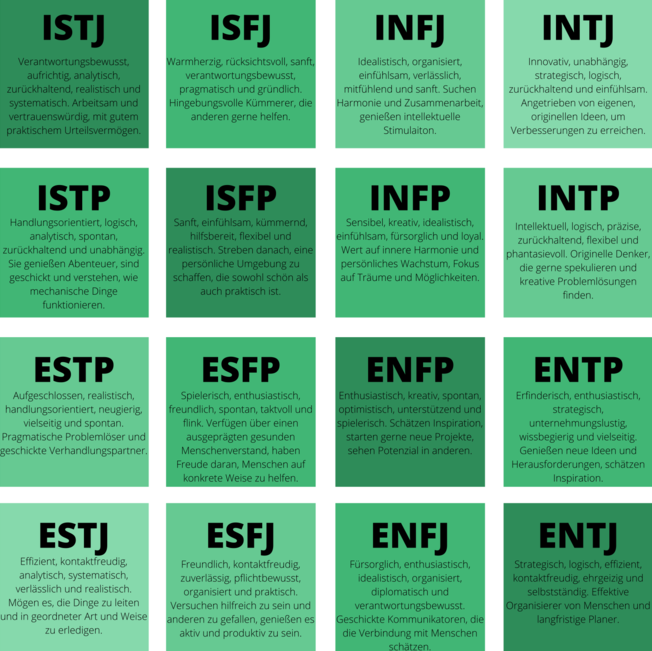
\includegraphics[width=0.35\textheight,angle=0]{img/Myers-Briggs-Typenindikator}}
	\caption[Myers-Briggs-Typenindikator]{Die 16 Persönlichkeitstypen nach Myers-Briggs}
	\label{img:mbti}
\end{figure}

Jeder einzelne Typ hat nach Myers-Briggs Auswirkungen auf Personen. \cite{myers_myers_2002} 
\begin{figure}[htbp!]
	\centering
	\fbox{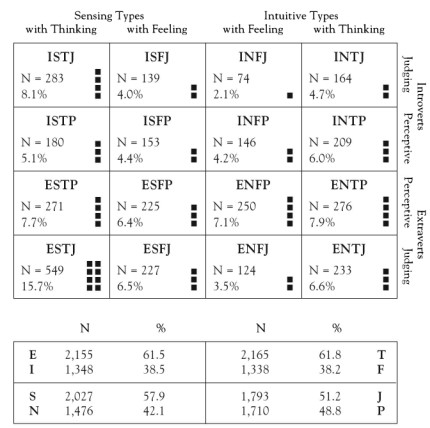
\includegraphics[width=0.35\textheight,angle=0]{img/distribution}}
	\caption[Verteilung der Myers-Briggs-Typen]{Verteilung der Myers-Briggs-Typen \cite{myers_myers_2002}}
	\label{img:mbti_distribution}
\end{figure}

\subsection{Studienrelevante Persönlichkeitscharaktere}
\subsubsection{Border Collie - ESTJ / ENTJ}
\begin{figure}[htbp!]
	\centering
	\fbox{
\includegraphics[width=0.2\textheight,angle=0]{img/Border_Collie}}
	\caption[Border Collie]{Border Collie}
	\label{img:Border_Collie}
\end{figure}
„Collie“ ist das schottisch-gälische Wort für „nützlich“. Sie sind logisch, entschlossen, kompetent und organisiert und bevorzugen eine Umgebung, in der sie ihre Intelligenz einsetzen, andere führen und aktiv gehalten werden können. Diese Kinder sind am glücklichsten, wenn sie die Möglichkeit haben, die Verantwortung zu übernehmen und sich zu messen. Sie genießen Herausforderungen, Debatten und die Interaktion mit einer Vielzahl von Menschen. Das Leben ist ein großer Wettbewerb, und sie sind entschlossen zu gewinnen.

\subsubsection{Elefant - ESFJ / ENFJ}
\begin{figure}[htbp!]
	\centering
	\fbox{
\includegraphics[width=0.2\textheight,angle=0]{img/Elephant}}
	\caption[Elefant]{Elefant \cite{knowAndLove}}
	\label{img:Elefant}
\end{figure}
Freundlich, aufgeschlossen und organisiert. Sie sind am glücklichsten, wenn sie anderen helfen, gesellschaftliche Veranstaltungen planen oder an Aktivitäten teilnehmen, an denen Menschen beteiligt sind – ALLE Menschen. Diese Kiddos bevorzugen ein harmonisches und kooperatives Umfeld mit viel Lob und Zuneigung. Im Leben dreht sich alles um echte Beziehungen und die Verbindung zu Menschen. 

Friendly, outgoing and organized. They're happiest when helping others, planning social events or participating in activities that involve people - ALL of the people. These kiddos prefer a harmonious and cooperative environment with lots of praise and affection. Life is all about genuine relationships and connecting with people.	\\
\subsubsection{Erdmännchen - INFP / ISFP}
\begin{figure}[htbp!]
	\centering
	\fbox{
\includegraphics[width=0.2\textheight,angle=0]{img/Meerkat}}
	\caption[Erdmännchen]{Erdmännchen \cite{knowAndLove}}
	\label{img:Elephant}
\end{figure}
Moralisch, sanft und sensibel mit einer kreativen und doch komplexen inneren Welt. Sie sind am glücklichsten in einer ruhigen, kooperativen und unterstützenden Umgebung, in der sie sinnvollen Dingen nachgehen können. Diese Kinder brauchen viel eingeplante Zeit allein, um ihre natürlichen Bauchgefühle zu verarbeiten und die Welt zu analysieren. Sie sind tief im Einklang mit den Gefühlen und Bedürfnissen anderer und neigen dazu, eine Friedensstifterrolle einzunehmen. Im Leben geht es darum zu verstehen, wie Menschen ticken. 

Moralistic, gentle and sensitive with a creative yet complex inner world. They're happiest in calm, cooperative and supportive environments where they can pursue meaningful matters. These kiddos need plenty of scheduled alone time to process their natural gut feelings and analyze the world. They are deeply in tune with others' feelings and needs and tend to take on a peacemaker role. Life is about understanding what makes people tick. \\	
\subsubsection{Panda - INFJ / INTJ}
\begin{figure}[htbp!]
	\centering
	\fbox{
\includegraphics[width=0.2\textheight,angle=0]{img/Panda}}
	\caption[Panda]{Panda \cite{knowAndLove}}
	\label{img:Panda}
\end{figure}
Intensiv privat, kreativ und ideenorientiert. Sie sind am glücklichsten, wenn ihre Bemühungen und einzigartigen Ideen anderen helfen, zu wachsen und zu lernen. Sie schätzen Autonomie und sind vertrauenswürdige, einzigartige, fähige und aufschlussreiche Personen. Diese Kinder bevorzugen eine ruhige Umgebung, in der sie in ihrer inneren Welt denken, verarbeiten und erschaffen können. Den Sinn hinter den Dingen zu verstehen, ist ihr Lebensziel. 

	Intensely private, creative and idea-oriented. They're happiest when their efforts and unique ideas help others to grow and learn. They appreciate autonomy and being trustworthy, unique, capable and insightful individuals. These kiddos prefer a calm environment where they can think, process and create in their inner world. Understanding the meaning behind things is their goal in life. \\
\subsection{Restliche Tiere}
Im folgenden wird zur Einordnung der bereits genannten Tiere in das gesamte Spektrum der Persönlichkeitstypen mit den Tieren, welchem keinem Kind in der Studie zugeordnet wurde, dargestellt.



\section{Computational Thinking} \label{sec:ct}
Um das informatische Denken der Kinder messen zu können, wurde mit den Kindern der Computational Thinking Test durchgeführt. Da die Kinder noch sehr jung sind, wurde deshalb die spezielle Variante für Jüngere, der sogenannte Beginners Computational Thinking Test, von den Kindern absolviert. Nach den Autoren des \acrshort{bctt}, \citeauthor{bcct}, ist die Fähigkeit des Computational Thinkings, eine kognitive Fähigkeit, welche für eine erfolgreiche Anpassung an die Zukunft wichtig ist, eine Kernfähigkeit. Dadurch, dass die Welt immer mehr den Schwerpunkt auf Technologie und Programmierungen legt, ist diese Fähigkeit des Computational Thinkings eine sehr kritische. Die Autoren des \acrshort{bctt} halten es für wichtig, dass Schüler und Schülerinnen in der Lage sein sollten, kritisch zu denken und komplexere Probleme lösen zu könne.\\
Die vier Kernelemente des Computational Thinkings sind Abstraktion, Dekomposition, Algorithmen und das Debugging.\\
\cite{bcct} 
\subsection{Beginners Computational Thinking Test}
Der \acrlong{bctt}, kurz \acrshort{bctt}, ist eine Weiterentwicklung des Computational Thinking Tests für Jüngere. Gemeinsam mit Experten wurde eine erste Version erstellt, welche mithilfe von Pilottests und Experten in eine zweite Variante verbessert wurde. Diese wurde anschließend an verschiedenen Schulen in Spanien durchgeführt.\\

Der \acrshort{bctt} ist in mehrere Segmente aufgeteilt. Insgesamt sind es drei große Kerngebiete, die wiederum in sechs verschiedene Aufgabengebiete aufgeteilt wurden, die der Test überprüft. Das erste Segment \glqq Sequences"' überprüft, ob die Kinder in der Lage sind, Sequenzen zu folgen. Dies ist das erste Kerngebiet des \acrshort{bctt}. Der zweite Abschnitt überprüft einfache Schleifen, der dritte Abschnitt überprüft verschachtelte Schleifen. Die beiden genannten Abschnitte bilden damit die Überprüfung für Schleifen. Das letzte Kerngebiet sind die sogenannten Conditionals. Dieses Kerngebiet wird von den drei Gebieten If-Then, If-Then-Else und While gebildet. Dort wird überprüft, ob die Kinder in der Lage sind, Anweisungen, welche an Bedingungen geknüpft sind, korrekt auszuführen.\\

Die Gebiete sind nicht gleich groß. Die Größe der Aufgabengebiete ist in der untenstehenden Tabelle dargestellt. Der größte Bereich wird vom Kerngebiet Schleifen gebildet, gefolgt von den Conditionals. Das kleinste Kerngebiet sind die einfachen Sequenzen.

\begin{table}[H]
	\centering
	\begin{tabular}{|l|l|}
		\hline
		Bezeichnung              & Anzahl Fragen \\ \hline
		Sequenzen                & 6             \\ \hline
		einfache Schleifen       & 5             \\ \hline
		verschachtelte Schleifen & 7             \\ \hline
		If-Then                  & 2             \\ \hline
		If-Then-Else             & 2             \\ \hline
		While                    & 3             \\ \hline
	\end{tabular}
	\caption{Anzahl Fragen pro Aufgabengebiet}
	\label{tab:distQuestions}
\end{table}

In Abbildung \ref{img:bcttQuestion} ist beispielhaft eine Frage eines Aufgabengebiets, hier das Gebiet der While-Conditionals, dargestellt. Eine Frage besteht immer aus einer Grafik und vier dazugehörigen Antworten, von denen nur eine richtig ist. Bei den Antwortmöglichkeiten sind die jeweiligen Anweisungen dargestellt, welche zur Lösung führen sollen. Die Aufgaben, bei denen neben Pfeilen auch andere Symbole verwendet werden, wie in der untenstehenden Abbildung dargestellt, beinhalten noch eine zusätzliche Anweisung für die Person, die den Test bearbeitet. 

\begin{figure}[H]
	\centering
	\fbox{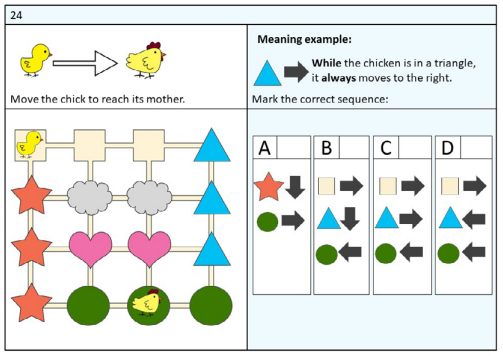
\includegraphics[width=0.4\textheight,angle=0]{img/bcttQuestion}}
	\caption[Beispielhafte Frage des \acrshort{bctt}]{Beispielhafte Frage des \acrshort{bctt}\cite{bcct}}
	\label{img:bcttQuestion}
\end{figure}

Die zweite Version des Tests wurde so abgeändert, dass auch Farbenblinde diesen Test durchführen können, weshalb die Felder in Abbildung \ref{img:bcttQuestion} mit Symbolen versehen wurden statt wie ursprünglich nur farbig dargestellt. Dies hat den Vorteil, dass zusätzlich der Test nicht zwingend in Farbe gedruckt werden muss, sondern auch in schwarz-weiß gut lösbar ist. \cite{bcct}

Der Test wurde wie bereits erwähnt an mehreren Schulen in Spanien angewendet. Insgesamt wurde eine Stichprobe von 299 Schüler und Schülerinnen an drei verschiedenen Schulen durchgeführt. Die Schüler und Schülerinnen waren in verschiedenen Klassenstufen, so dass der Test die Klassen 1,2,4,5 und 6 abdeckte. Für die Studienarbeit sind die Daten der Schüler und Schülerinnen relevant, welche die zweite Variante des \acrshort{bctt} durchführten. Die Ergebnisse nach \citeauthor{bcct} sind in der untenstehenden Tabelle dargestellt. Für die Studienarbeit nicht relevante Daten wurden aus Gründen der Übersichtlichkeit nicht übertragen.

\begin{table}[H]
	\centering
	\begin{tabular}{|l|l|l|l|}
		\hline
		\rowcolor[HTML]{C0C0C0} 
		Klassenstufe & N  & durchschnittliches Ergebnis & Standardabweichung \\ \hline
		2            & 18 & 14.278                      & 2.445              \\ \hline
		4            & 28 & 21.286                      & 1.922              \\ \hline
		6            & 25 & 21.280                      & 3.542              \\ \hline
	\end{tabular}
	\caption[Statistiken des \acrshort{bctt}]{Statistiken des \acrshort{bctt} nach \citeauthor{bcct}}
	\label{tab:statisticsBCTT}
\end{table}


\section{Torrance Tests}{
	\label{sec:torrance_tests}
	\begin{figure}[H]
		\centering
		\fbox{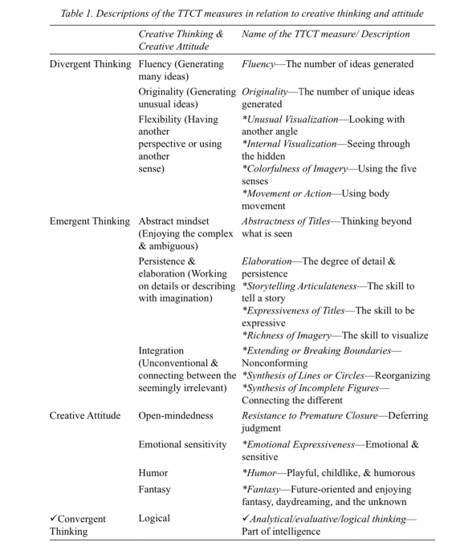
\includegraphics[width=0.4\textheight,angle=0]{img/ttct}}
		\caption[Relation von TTCT-Maßnahmen]{Relation von TCTT-Maßnahmen gegenüber kreativem Denken und kreativer Haltung \cite{Kim2016}}
		\label{img:ttct}
	\end{figure}
}
